\documentclass[10pt,twocolumn,letterpaper]{article}

\usepackage{cvpr}
\usepackage{times}
\usepackage{epsfig}
\usepackage{graphicx}
\usepackage{amsmath}
\usepackage{amssymb}
\usepackage{subfigure}
% Include other packages here, before hyperref.

% If you comment hyperref and then uncomment it, you should delete
% egpaper.aux before re-running latex.  (Or just hit 'q' on the first latex
% run, let it finish, and you should be clear).
\usepackage[breaklinks=true,bookmarks=false]{hyperref}

\cvprfinalcopy % *** Uncomment this line for the final submission

\def\cvprPaperID{****} % *** Enter the CVPR Paper ID here
\def\httilde{\mbox{\tt\raisebox{-.5ex}{\symbol{126}}}}

% Pages are numbered in submission mode, and unnumbered in camera-ready
%\ifcvprfinal\pagestyle{empty}\fi
\setcounter{page}{1}
\begin{document}

%%%%%%%%% TITLE
\title{Image Colorization using Cold diffusion with Latent Diffusion Models}

\author{Francesco Boraso\\
{\tt\small francesco.boraso@studenti.unipd.it}
% For a paper whose authors are all at the same institution,
% omit the following lines up until the closing ``}''.
% Additional authors and addresses can be added with ``\and'',
% just like the second author.
% To save space, use either the email address or home page, not both
\and
Marco Brigo\\
{\tt\small marco.brigo@studenti.unipd.it}
\and
Fabio Pantaleo\\
{\tt\small fabio.pantaleo@studenti.unipd.it}
}

\maketitle
%\thispagestyle{empty}

%%%%%%%%% ABSTRACT
\begin{abstract}
Image colorization aims to add realistic colors to grayscale images, which is challenging due to its inherently ill-posed nature. While diffusion models have demonstrated impressive results on this task, they typically require extensive computational resources and training data. We have implemented an efficient colorization approach, thanks to Stable Diffusion that works in latent space rather than raw pixels, based on Cold Diffusion that achieves results with significantly reduced training requirements. Our method leverages a pre-trained Stable Diffusion model and combines it with LoRA for parameter-efficient fine-tuning and BLIP-generated captions for semantic guidance. We trained the UNet model of the pre-trained model on the Imagenette dataset with targeted augmentations, in order to enhance vivid colors and avoid desaturation and washed-out results. Then we tested our model on a 5K test set of MS-COCO.  Our code is available at \href{https://github.com/MarkBridge11/Image-Colorization-VCS2425}{https://github.com/MarkBridge11/Image-Colorization-VCS2425}
\end{abstract}

%%%%%%%%% BODY TEXT
\section{Introduction}

Image colorization involves generating plausible colors for grayscale images, presenting a fundamentally ill-posed problem since multiple color solutions could be valid for a single grayscale input. The main challenges arise from this inherent ambiguity, where objects can have multiple valid colors, and the regression-to-mean problem when using standard losses. Traditional approaches using direct regression losses tend to produce desaturated results as they average out multiple possible colors to minimize error. While GANs attempt to address this through adversarial training to maintain color vibrancy, they suffer from mode collapse and training instability. These challenges require solutions that can effectively model multiple color possibilities while maintaining both local consistency and global semantic understanding. \\
\indent Recent advances in diffusion models have shown promising results for image colorization, particularly we found interesting the work of the paper ~\cite{ReferencePaper} that we’ve tried to implement. Their approach stands out for combining powerful text-guided control with efficient implementation. By leveraging Latent Diffusion Models, it achieves high-quality colorization while requiring less computational resources than pixel-space diffusion methods. The method provides flexible control through text prompts but can also operate automatically, making it practical for real-world applications. Additionally, it outperforms previous methods in terms of both quality and controllability, as demonstrated through quantitative metrics and user studies.
\\
\indent 
In this work, we implement and adapt their approach with several practical considerations:
\begin{itemize}
\item We utilize LoRA (Low-Rank Adaptation) for efficient fine-tuning of the Stable Diffusion U-Net, reducing the number of trainable parameters while preserving model capacity.
\item We incorporate BLIP-generated captions to provide semantic guidance during the colorization process, helping ensure contextually appropriate colors.
\item We train on the Imagenette dataset with targeted augmentations designed to encourage more vivid colorization and prevent the desaturation problems common in colorization models. Also like mentioned in the work of reference paper, we’ve filtered out grayscale and low-saturation samples.
\item A more thought out scheduling procedure that modified the timestep calculation making training more effective, in order to challenge the model to color more.

\end{itemize}	

%------------------------------------------------------------------------
\section{Related works}

%-------------------------------------------------------------------------
\subsection{Automatic Colorization}


Fully automatic colorization methods aim to colorize grayscale images without user input and earlier approaches suffered from desaturated results due to the ill-posed nature of the task. This led to solutions such as distribution prediction [Larsson et al. 2016a; Xia et al. 2022] and deep learning-based paradigms like CIColor ~\cite{CI}. More recent techniques leverage generative models, including GANs~\cite{GAN}~\cite{GAN1} and denoising diffusion models ~\cite{DDM}
\\
\indent
On the other side we have user guided colorization that has also given interesting results.  Levin et al. [2004] ~\cite{Levin} and UGColor [Zhang et al. 2017] ~\cite{UGColor} proposed user interactions directly in the image using clicks or color scribbles respectively. Vitoria et al. [2020] first analyze the contents of an image and segment it into the different objects, next they use a fusion module to combine the representation and obtain a valid colorization.



%-------------------------------------------------------------------------
\section{ Dataset}

We trained our model on Imagenette (\href{https://github.com/fastai/imagenette}{https://github.com/fastai/imagenette}), a smaller curated subset of ImageNet ~\cite{ImageNet}  classes. While the original paper used the full ImageNet dataset, our approach focused on leveraging the strong generative capabilities already present in the pretrained Stable Diffusion model. By using LoRA fine-tuning, we could effectively adapt these pretrained weights with a much smaller dataset, balancing computational efficiency with training effectiveness. For validation during training, we used a small streaming subset of ImageNet. For validation during training, we used a small streaming subset of ImageNet.
\\
\indent
To assess the model’s ability to generalize, we tested it on a 5,000-image subset of MS-COCO, a dataset known for its diverse, real-world imagery, following the evaluation protocol of the reference paper. By evaluating performance on MS-COCO, we ensured that our model was not overfitting to Imagenette-specific features and could effectively colorize images from a different distribution.

\subsection{Datasets preprocessing}
Following the recommendations from the reference paper we have preprocessed the dataset. Firstly we filtered out grayscale images and low-saturation samples. We decided to increase their saturation threshold to 0.18 to ensure that the model was trained on meaningful color variations. 
\\
\indent
To improve generalization and enhance vividness, we applied data augmentation to 10\% of the images. This included:
gaussian blur
,random contrast variation 
,random brightness adjustment 
,chromaticity increase.

Then to further encourage the network to learn color representations effectively, we artificially increased the saturation and chroma boost of 40\% of the dataset, amplifying color intensity and diversity. This aggressive approach was justified by the preliminary results which were very grayish and desaturated.
\\
\indent
Finally we normalized all images to a mean of 0.5 and a standard deviation of 0.5. This range was used to match the VAE input requirements.
\\
\indent
For what concerns the training dataset, as suggested by the reference paper to enhance training, we have captioned the Imagenette dataset using BLIP (Bootstrapping Language-Image Pre-training). This provided automatic text descriptions for each image, which were used during training to guide the colorization process. Following the paper's approach, we randomly removed captions for 10\% of the training samples to make the model more robust and capable of colorizing images even without text guidance. We decided to not include captions in the preprocessing of the test set since the best results that they were achieving were by using only negative prompts.

%-------------------------------------------------------------------------
\section{Method}
Our approach to image colorization combines three key components: Cold Diffusion, LoRA (Low-Rank Adaptation), and BLIP-based text conditioning. Cold Diffusion provides the foundation by treating colorization as a deterministic degradation process rather than a noise-based one, making it particularly suitable for the colorization task where we want to preserve structural information while adding color.


\subsection{LoRA}
LoRA (Low-Rank Adaptation of Large Models)  ~\cite{LoRA} is a technique that enables efficient fine-tuning of large neural networks by updating only a small subset of parameters. Instead of modifying all layers of a pre-trained model, LoRA introduces low-rank decomposition matrices into key layers, significantly reducing the number of trainable parameters while maintaining performance. 
The low-rank updates are defined as: \begin{math}
W = W_0 + BA
\end{math}
, where \begin{math}W_0 \end{math} is the frozen pretrained weight matrix, B and A are the low-rank decomposition matrices, and their product BA represents the update to the weights. This decomposition typically uses a rank r much smaller than the original weight dimensions, making it highly efficient. 
In our implementation, we apply LoRA to the U-Net backbone of Stable Diffusion, targeting the cross-attention blocks and feed-forward components. This allows us to: reduce the trainable parameters from hundreds of millions to just a few million, maintain the pretrained model's understanding of image structure and semantics, specifically adapt the model for the colorization task, achieve faster training and lower memory requirements. 

\subsection{Stable diffusion model}
The stabilityai/stable-diffusion-2-1 ( \href{https://huggingface.co/stabilityai/stable-diffusion-2-1} {https://huggingface.co/stabilityai/stable-diffusion-2-1}) model is based on Latent Diffusion Models (LDMs)  ~\cite{Rombach}. It is designed to efficiently generate high-quality images while reducing computational demands, leveraging three key components: a Variational Autoencoder (VAE), a U-Net with a diffusion process, and text embeddings via CLIP.
\\
\indent
Unlike traditional diffusion models that operate directly in pixel space, Stable Diffusion first compresses images into a lower-dimensional latent space using a VAE. The encoder E(x) transforms an image x into its latent representation z, reducing the computational complexity required for processing. Once the diffusion process is completed, the decoder D(z) reconstructs the image from the latent representation, ensuring high fidelity while avoiding unnecessary high-frequency details.
At the core of the model lies a time-conditional U-Net, responsible for the denoising process. During training, a forward diffusion process gradually adds Gaussian noise to the latent representation over multiple timesteps t. The U-Net then learns to reverse this process by predicting and removing the noise step by step, progressively refining the image until a clear representation is restored. To further improve the quality of generated images, the model employs classifier-free guidance, which enhances the generation process based on additional conditioning inputs.
\\
\indent
Stable Diffusion also supports text-to-image synthesis, integrating CLIP text embeddings to guide the generation process. A cross-attention mechanism enables the U-Net to align image generation with textual descriptions, allowing precise control over the final output. By leveraging this structured approach, the model achieves efficient and high-quality image synthesis while maintaining flexibility in conditioning and generation control.


\subsection{Training Algorithm}

Our training implementation follows the core approach from "Diffusing Colors: Image Colorization with Text-Guided Diffusion" (see Figure \ref{fig:training}, while introducing some modifications to the timestep sampling strategy. The training process operates in the latent space of a pre-trained Stable Diffusion model, where we leverage both its VAE for efficient latent encoding and its UNet backbone through LoRA fine-tuning.
For each training iteration we used their training algorithm as specified in the Algorithm 1 of Implementation Details in the Supplementary Material of the reference paper:

\begin{enumerate}
\item Both the RGB image and its grayscale version are encoded through the pretrained VAE, yielding latent representations $\mathit{z_{rgb}}$ and $\mathit{z_{gray}}$
\item A timestep t is sampled (we experimented with different sampling strategies, detailed below)
\item These latents are linearly interpolated based on t: \begin{math}z_t = (1-t) × z_{gray} + t * z_{rgb} \end{math}
\item The UNet with LoRA predicts the color residual given \begin{math}z_t \end{math}, t, and the BLIP-generated caption
\item The loss is computed as the Mean Squared Error between the predicted and true color latents
\end{enumerate}

\begin{figure}[t]
    \centering
    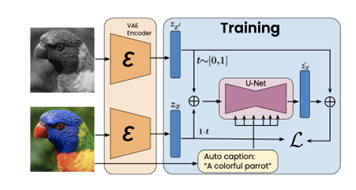
\includegraphics[width=0.8\linewidth]{TrainingAndInference.png}
    \caption{Overview of the training phase.}
    \label{fig:training}
\end{figure}

\begin{figure}[t]
    \centering
    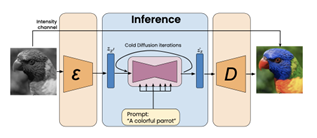
\includegraphics[width=0.8\linewidth]{TrainingAndInference_2.png}
    \caption{Overview of the inference phase.}
    \label{fig:inference}
\end{figure}
The original paper samples t uniformly from [0,1], which resembles traditional diffusion processes where noise is gradually injected into the image. However, we found that this uniform sampling doesn't optimally address the colorization task. Instead, we tried several dynamic sampling strategies that evolves during training, for example:
\begin{itemize}
\item Initially uses uniform sampling to learn the full range of color interpolation
\item Gradually shifts towards lower t values after specific number of steps (approximately half of training)
\item This biased sampling forces the model to focus on more challenging cases where the input is closer to grayscale, improving its ability to add color from minimal information
\end{itemize}

We explored different timestep sampling strategies because our initial experiments using the uniform sampling from the original paper often resulted in desaturated and washed-out colorizations. The key issue was that with uniform sampling from U(0,1), the model was primarily learning to refine colors for high t values, where much of the color information was already present in the interpolated image. When combined with the MSE loss, as suggested by the reference paper, this led to a problematic convergence behavior: the model was learning to make minimal adjustments to the input, effectively doing almost nothing, especially for high t values where the interpolated image was already close to the target. This resulted in the model failing to learn how to effectively add color information when needed, leading to gray and washed-out results. By modifying the sampling strategy to focus more on lower t values during training, we forced the model to learn the more challenging task of inferring and generating colors from minimal information, rather than just making small refinements to already-colorful inputs.

\subsection{Cold Diffusion for Image Colorization}
Cold diffusion is a deep learning technique derived from the diffusion models. In normal diffusion models, degradation is introduced through random Gaussian noise applied to the image. The key difference in cold diffusion is that the degradation of the image is done through a deterministic approach which in our case is desaturation (gradually removing the color information in the image). This allows the model to retain the luminance information of the image and the model should achieve much better results on this task.
\\
\indent
Desaturation as a degradation method is a more effective and interpretable approach compared to Stable Diffusion as we don’t need to worry about the structural information to focus solely on the coloring of the image. This leads to a reduction in training complexity and justifies why we used such a small dataset.
\\
\indent
Cold Diffusion is a novel framework~\cite{Cold}, challenging the traditional assumption that Gaussian noise is a necessary component of diffusion-based generative models. Instead of adding random Gaussian noises to images, Cold Diffusion generalizes the diffusion process to arbitrary and even deterministic image transformations, such as blurring, inpainting, downsampling, masking and in our case removing color.
\\
\indent

Cold Diffusion replaces noise with a deterministic degradation function D(x,t), which applies controlled transformations to an image at different severity levels and a restoration model R(x,t) is trained to invert these transformations. Moreover a new sampling approach is introduced as an improved sampling method for Cold Diffusion, addressing the instability of traditional sampling techniques when using deterministic degradations. Unlike noise-based diffusion, Cold Diffusion relies on structured, reversible transformations (e.g., blur, inpainting, downsampling) and requires a different iterative reconstruction approach. 
\\
\indent
Given a Degraded Sample $x_t $ (the most transformed version of the image), a Trained Restoration Model (x,t) which learns to invert transformations, a Degradation Function D(x,t) and Number of Steps to controlling how many iterative refinements are performed, the algorithm steps are:

\begin{enumerate}
\item Initialize the degraded image $x_t $, which is the most severely transformed version of the original image.
\item Iterate from step t down to 1:
\begin{itemize}
\item Use the restoration model to estimate the original image: $ \hat{x}_0 = R(x_s, s) $
\item Apply a correction step to refine the update: \begin{math} x_{s-1} = x_s - D(\hat{x}_0, s) + D(\hat{x}_0, s-1) \end{math} 
\item This equation ensures that the reconstruction does not deviate too much from the expected transformation sequence.

\end{itemize}

\end{enumerate}

\subsection{Inference Algorithm}
The inference process (see Figure \ref{fig:inference})follows the guideline of the reference paper. It’s an iterative colorization procedure that operates in the latent space. Given a grayscale input image, the algorithm refines a latent color representation step-by-step using a fine-tuned UNet model, conditioned on optional text prompts for guided colorization.
The main components of the inference algorithm are:

,VAE Components: Encoder E(x) and Decoder D(z)
,UNet Model: Pre-trained model for latent color prediction
,Grayscale Image: \begin{math}x' \in \mathbb{R}^{H \times W}\end{math}
,Number of Iterations: T, controlling the refinement process
,Optional Text Prompts(
	Positive Prompt c (to guide the desired colors)
	,Negative Prompt $c^{\prime} $ (to suppress undesired colorization)
)
,Guidance Scale: s, determining the strength of the prompt influence
Color Scale: $s^{\prime} $, adjusting the final color intensity


Inference Algorithm:
\begin{enumerate}
\item Latent Encoding:
The grayscale input image  $x^{\prime} $ is encoded into the latent space using the VAE encoder:
$z_{t^x} = z_{x^{\prime}} = E(x^{\prime})$
\item Iterative Refinement: For each timestep t from T down to 1:
\begin{itemize}
\item Predict the color residual using the UNet model for both positive and negative prompts: \begin{math} \hat{\Delta}_{c}, \hat{\Delta}_{c^{\prime}} = \text{UNet}(z_{t^x}, t, c), \quad \text{UNet}(z_{t^x}, t, c^{\prime}) \end{math}
\item Apply classifier-free guidance to enhance the predicted colors: \begin{math} z_x = z_{t^x }+ \hat{\Delta}_{c} + s \cdot (\hat{\Delta}_{c} - \hat{\Delta}_{c^{\prime}})\end{math} 
\item Update the latent representation iteratively: \begin{math} z_{t^x }= z_{t^x }+ \frac{1}{T} (z_x - z_{x^{\prime}})\end{math} 
\end{itemize}
\item Final Colorization:

\begin{itemize}
\item Apply a scaling factor to adjust the final color intensity: \begin{math} z_x = z_{x^{\prime}} + s^{\prime}\cdot (z_x - z_{x^{\prime}})\end{math} 
\item Decode the final latent representation into pixel space to obtain the colorized image: \begin{math}x = D(z_x)\end{math}
\end{itemize}
\end{enumerate}

This inference process ensures that the grayscale image is progressively colorized in a controlled manner, leveraging the expressiveness of diffusion models and the efficiency of latent-space processing. The use of classifier-free guidance enables flexible user control over the final colorization results while maintaining the model’s generative quality.

%-------------------------------------------------------------------------
\subsection{Alternative approaches tried}

Before adopting our final Cold Diffusion approach, we experimented with several alternative models for image colorization, including PixelCNN, GANs, ControlNet, and ResNet. While these methods have been successfully applied in generative modeling and image processing, they did not meet our performance expectations due to computational constraints or colorization quality issues.

\begin{itemize}
\item PixelCNN is an autoregressive model that generates images pixel by pixel based on conditional probabilities. While it ensures high-quality local dependencies, its sequential nature makes training too slow, making it impractical for us.
\item GANs use a generator and a discriminator in an adversarial framework in which the generator provides a potential coloring for the image and the discriminator tries to distinguish it from the dataset. Also in this case, training was computationally expensive, and we encountered mode collapse, where the model generated repetitive or limited color distributions instead of diverse and realistic results.
\item We also experimented with using ResNet as an encoder to extract latent representations from grayscale images, followed by upscaling for colorization. While effective at feature extraction, this approach led to desaturated outputs due to L2 loss favoring mean color predictions. Furthermore, the lack of a probabilistic framework limited color diversity. 
\item We also explored ControlNet ~\cite{ControlNet}, which adds conditional control to pretrained diffusion models. Applied to the UNet, it creates a trainable copy of the encoder layers and middle block, keeping the original model frozen. ControlNet receives the latent image, timestep, text embeddings, and an extra conditioning input—Canny edges of the grayscale image. Its outputs are merged with the main model via zero-initialized convolutions, ensuring gradual learning. However, the results were worse than our final approach.
\end{itemize}

Given the limitations of these approaches, we turned to Cold Diffusion, which provided a more interpretable and efficient solution for image colorization. Despite its initial complexity, Cold Diffusion allowed for accurate and vibrant color restoration within our computational constraints.

\begin{figure*}[h]
\centering
\begin{subfigure}
  \centering
  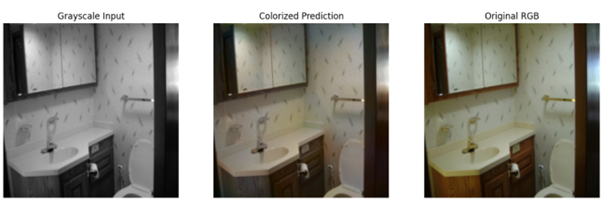
\includegraphics[width=1\textwidth]{results.png}
\end{subfigure}
\vspace{2mm}
\begin{subfigure}
  \centering
  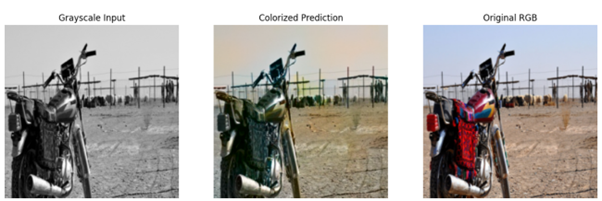
\includegraphics[width=1\textwidth]{results2.png}
\end{subfigure}
\caption{Qualitative comparison of our proposed method.}
\label{fig:results}
\end{figure*}

\section{Experiments and Results}
Our training pipeline incorporated MSE loss, text embeddings, and a sampling strategy for the diffusion timestep t. However, we encountered a well-known challenge in colorization tasks: the tendency of the model to generate grayscale or desaturated outputs. This problem accompanied us throughout the project, making various attempts to avoid it.We have trained the model for:
,3 epochs using a A100 GPU
,batch size of 16 images
,learning rate of 1e-5
,AdamW as optimizer.


A key issue was that MSE loss prioritized structural reconstruction over colorization, causing the model to focus more on preserving image details rather than accurately predicting chromatic information. In fact, since we were exploiting the generational power of the pre-trained model, the MSE loss quickly went down to lower values. For this reason we decided to incorporate other losses, weighting less the MSE (we decided to keep that to maintain the structure of the images but with less relevant since it was already producing structure-speaking, good results). We have tried to combine the MSE with the following loss functions:

\begin{itemize}
\item Saturation loss: Measures the difference in the Saturation (S) channel between two images, typically in HSV color space.
\item LPIPS  ~\cite{LIPS}: A perceptual loss that computes feature differences between images using deep network activations (e.g., VGG, AlexNet)
\end{itemize}

Nonetheless none combination was a game-changer, in fact they were not drastically changing the information as also confirmed in the paper ~\cite{Ballester}.
We experimented with different sampling strategies for t during training, but none significantly improved the colorization quality. Instead, we observed that higher t values (corresponding to stronger degradation) reduced the effort required by the model to restore color, which led to a trivial solution where the model converged to applying minimal or no colorization.
One promising result was the effectiveness of text embeddings in guiding the model’s predictions. While standard training led to desaturated outputs, incorporating text-based conditioning significantly improved color accuracy and semantic coherence. This suggests that explicit textual guidance can help counterbalance the limitations of pixel-based losses by enforcing stronger semantic constraints on colorization.
As explained before we tested our model on a subset of the COCO MS dataset, this ensures that the images are completely different from the training data used. Below we include some of the results of our final model using only MSE loss.


We observed that the model tends to produce perceptually realistic results when handling light colors and nearly uniform scenes, but struggles with more vibrant colors such as red, green, and others.
To quantitatively assess the quality of the colorized images, we employed the FID (Fréchet Inception Distance) metric, computed on the test set. FID is a widely used measure for evaluating the quality of generated images by comparing the feature distributions of real and generated images, extracted using a pretrained Inception v3 network. Lower FID values indicate better image quality, with a score of 0 representing an exact match. State-of-the-art models typically achieve FID scores ranging between 5 and 50, depending on the dataset and the model's ability to generate realistic images. A score above 50, like ours, suggests substantial room for improvement, particularly in terms of color accuracy and semantic consistency.
\\
\indent
Our model achieved an FID score above 70 (77.4), which is relatively high. This indicates that while the model can generate perceptually plausible results in certain scenarios, the overall quality of the colorization is suboptimal. A high FID score reflects a significant discrepancy between the generated and real images, both in visual appearance and feature distribution. This highlights the need for improvements, especially in handling complex or highly saturated color regions.


\section{Conclusion}
In this report, we have presented a lightweight approach to image colorization, based on state-of-the-art techniques and enhanced through various improvements such as BLIP captioning, LoRA for more efficient training, and a more effective training procedure utilizing scheduling for the t values. We have experimented with multiple approaches, as described above, to refine the model's performance. However, after careful consideration, we believe the primary limitation likely lies in the scale of the dataset and the duration of training. Such an approach would enable the model to better capture the complexities of color distribution, particularly in challenging regions with vivid or saturated colors, ultimately leading to higher fidelity and more semantically coherent results. Addressing this limitation could be the key to unlocking the full potential of the model, which could have led us to the same result as the reference paper. 

%-------------------------------------------------------------------------
\clearpage

{\small
\bibliographystyle{ieee_fullname}
\bibliography{egbib}
}

\end{document}
